%! Suppress = MissingImport
\section{Detailed Workflow}\label{sec:detailed-workflow}

This section is going to detail the new proposed workflow.
It's going through each step, by detailing exactly what have been changed,
modified or removed.
Some tools, such as Cucumber or Gitlab, will be directly integrated to the
step description, in order to provide concrete examples of the process
implementation.

To keep this section straightforward and focused on the workflow, some
implementation details or advices will be omitted and moved to the next
sections of this chapter.

\subsection{Design \& Specs}\label{subsec:design-specs}
This first step of design and specifications is inherited from the
document-oriented approach of the waterfall methodology and V-model.
This step haven't really been improved nor modified and basically remains the
same.

The analysts will work with the stakeholders to understand their business
needs and formalize their requirements.
The architect will then design a solution that should be able to solve the
problem.
They will finally write the specifications of the solution that will fulfill
the global business needs.

This step is where the client is mostly involved during the workflow, because
once he validated the documentation, it should be a standalone source of
information for the whole development process.

% TODO populate requirements and solution specification in ALM tool
% TODO split into subsubsection if it's considered as too short

\subsection{Test Strategy}\label{subsec:test-strategy}
The test strategy step is also inherited from the traditional methodologies.
The manner or tool used to design a test strategy won't really be changed.
However, since the context in which the tests are going to be written and
executed will be different from the traditional one, we're going to mention
some important points.

\subsubsection{Previous context}
Before, in traditional methodologies, the test strategy simply consisted of
defining how to test each part of the specification, in an abstract way.
There were various information, such as the dataset or the account type to use
but the detailed steps weren't written yet.
It is a kind of feasibility study on how to test the application, to ensure
that every feature can be correctly tested.

When writing the test cases, the author can assume that, when the test will
be executed, the implementation phase will be completed and therefore all the
features defined in the specification will be available.
The order of test writing wasn't a problem too, because the test will be
executed only once every tests will be designed, so there's no need of
prioritization.

\subsubsection{New context}
In the new workflow, the context is different from the previous one.
Tests are not executed at the end anymore, but throughout the development
process.
Indeed, a new test is written, it is intended to be used as an executable
specification and drive the implementation phase.
This will provide a quick feedback on the feature itself but also on the test
format.

At first glance, the ordering doesn't really matter since there should be
enough information regarding the scenario and the global documentation to
implement the feature.
Well in fact, the problem lies on the feedback duration.
Here is an example with a small set of modules and their dependencies.

\begin{figure}
    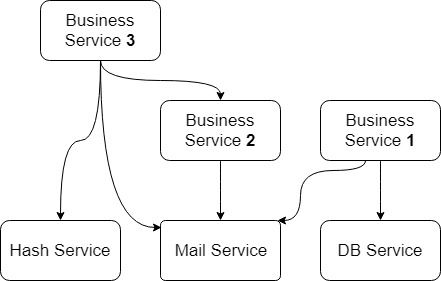
\includegraphics[width=\textwidth]{../../resources/images/solution/module_dependencies.png}
    \centering
    % TODO fix position with the related text
\end{figure}

In this figure, the \textit{Business Service 3} depends on 2 common modules
and 1 other business service.
When writing the scenarios, all the information will be available to the tester,
thanks to the comprehensive specification, so there won't be any problem when
writing it.

However, when the scenario will be submitted to the developers, they will
need all the dependent modules to be implemented in order to implement the
\textit{Business Service 3}.
If this scenario is written first, then it will take days to have the feedback.

Furthermore, they will have to work on modules that don't have their
scenarios written.
Which means that they either have to wait for them or start the
implementation without the tests, which would be like working the old
traditional way we want to avoid.

As mentioned earlier, one of the key concept of BDD is communication and it
allows the team to have a quick feedback during the development process.

\subsubsection{Defining the right strategy}
In order to reduce the feedback duration and let the tests drive the
implementation, the test strategy should not only cover how to test the
solution but also in which order they should be written.

The approach should be following the agile principle about building
progressively the application, step by step.
Every new test will produce a new feature or service and will add value
to the application.
The prioritization should be made regarding the importance of the module and
its dependencies, in order to have test that are easy to implement.

A feature that has a lot of unimplemented dependencies won't be a great
candidate at the beginning, because it will require too much effort to make
it pass.
These dependencies, usually common services, should therefore be tested
and implemented first, to then be able to implement business modules.
The important idea here is to always try to produce a test, which is also an
executable specification, that is easily doable at the time it's released.

But there are some cases where it's okay to produce it even if it's not
quickly doable.
For example, when a module is implemented at 95\%, it's preferable to write
the last test, so the testers can complete this module and move to another one.
The developers will simply ignore this test for now and will take a look at
it when its dependencies will be correctly implemented.

The test strategy can also be discussed with the client.
This can be very useful during the prioritization,when defining the set of
core modules and services.
Both the client and analysts will share the same vision and understanding of
what's vital to the application and what is less important.

\subsection{Acceptance Test Kickoff}\label{subsec:acceptance-test-kickoff}
This new step occurs right after the validation of the test strategy.
Here, the team is going to set up the base of the acceptance tests that will
be used for the rest of the workflow.

In absolute, this step could have been omitted and its content included in
the test writing steps.
However, since the acceptance scenarios are going to be at the center of the
development process, they must be strong and reliable.
Therefore, they have a dedicated step to set up everything and validate the
scenario base before starting using it.

\subsubsection{Define the vocabulary}
The vocabulary used to write the scenarios is critical.
A scenario must be self explanatory, have clear intents by describing the
expected behaviour.
Hence it must use domain-specific words, so the analysts feel comfortable
when writing it and share the same words with the developers.

The definition of the vocabulary must not be done by only one side (analysts
or developers).
If so, the other team is likely to misunderstand the scenario or to miss the
important business aspect of a feature.
This would be just like in the traditional methods, where they were
interpreting and implementing a specification, without clearly understand it.

Therefore during this step, at least the tech lead should be present with the
analysts, but it would be better to have several other members, such as the
architect or another developer.

The presence of the developers is very important because they will have to
implement the code of the scenarios.
Hence they can slightly adapt the vocabulary and the sentence format so it
will be easier to write and automate.

\subsubsection{Write the first scenarios}
Once the vocabulary is defined, the first scenarios can be written.
During the test strategy, the ordering have already been defined, so the
first scenarios to write are already known.
These scenario are going to be used as sample, to get familiarized
with vocabulary and adjust it if necessary.

During this phase, one important point to address is to define the correct
abstraction and granularity of the scenarios.
As said earlier, scenarios must be self explanatory and easily understood by
both the analyst and developer.

If the scenario is too abstract, then it will allow more interpretation and
the result is likely to diverge from the expected result of the writer.
In addition, it won't really \textit{drive} the implementation as it will be
too high level.

A contrario, a very detailed scenario will be less readable and will probably
lose its \textit{domain} aspect, as it's likely to simply specify the
technical requirements instead of describing a behavior.
A scenario too technical will also make the analyst less comfortable with, as
it won't use its domain words.

\subsubsection{Validate the base}
In order to validate the sample scenarios, the developers will write their
code and execute it with the analysts.

The first implementations will validate that the vocabulary used and the
scenario format is indeed executable and easily automated.
These implementation will be reused and extended throughout the development
process, so they must be validated as early as possible.

Once implemented, the scenario are going to be executed and validated using
some sort of shadowing.
Shadowing is a technique of knowledge transfer, where a new incomer will learn
how a person does its job, by observing him and doing the same thing and
eventually replace him.
The previous person will validate the knowledge transfer by staying with the
new incomer but letting him actually do the job.

In this case, it's not really shadowing, because the tests are not going to
learn from the testers.
However, when the tests will be executed, the testers will watch what they
are actually doing and see if the tests are valid and their verification
relevant.

This validation is a very important step to make the team confident regarding
their test implementations.
If these tests are correct, then the new tests produced using the same format
and vocabulary will also be reliable and trustful.

\subsection{Test Writing}\label{subsec:test-writing}
% TODO scenario format (UI / API / low-level) - move this to next section ?
% TODO how to implement the steps
% TODO we can use NoraUI
% TODO we can improve it for the API testing
% TODO backlog filling
% TODO new vocabulary must be discussed with the tech lead
% TODO use of the ALM to still have a coverage
% TODO test that can't be automated

\subsection{Implementation}\label{subsec:implementation}
% TODO consumes from the backlog
% TODO work in TDD
% TODO work in PP
% TODO ci setup
% TODO use a merge request
% TODO feedback on the scenario if needed
% TODO WIP tag to have an overview of the progress

\subsection{Qualification}\label{subsec:qualification}
% TODO reuse the same scenario
% TODO validate at least one time each scenario ..
% TODO .. or validate enough important scenario to trust the others
% TODO improve test reports to add some proof (screnshots, logs, DB dump etc.)
% TODO describe the bug workflow
% TODO run the test that cannot be automated